\documentclass{article}
\usepackage{multicol}
\usepackage{graphicx}
\usepackage{float}
\usepackage{hyperref}
\title{RescueLink: A Mobile Application for Victim Localization in Emergency Situations}
\author{
    Paolo Palumbo \\ 
    \href{mailto:p.palumbo3@studenti.unipi.it}
        {p.palumbo3@studenti.unipi.it}
    \and Ettore Ricci \\ 
    \href{mailto:e.ricci32@studenti.unipi.it}
        {e.ricci32@studenti.unipi.it}}
\begin{document}
\maketitle
\begin{abstract}
In emergency situations, rapid
and accurate localization of potential 
victims is crucial for effective rescue operations.
This project presents an innovative Android 
application using Bluetooth Low Energy (BLE) 
technology, trilateration, and GPS to enhance 
victim localization. 
The system ustilizes an ah-hoc BLE network
to share information between devices and 
computes the victim's position using trilateration 
when GPS is not available.
\end{abstract}
\begin{multicols}{2}
\section{Introduction}
During emergency situations such as natural 
disasters, fires, and large-scale accidents, 
the timely and accurate localization of 
potential victims is foundational to effective
rescue operations. 
Current methods usually rely on visual searches
and may be ineffective in low-visibility scenarios.
Due to the influence of modern technology, 
the majority of people carry smartphones and other
BLE-enabled devices with them. 
This project aims to leverage these devices to
localize victims in emergency situations.
A version of the application can also be installed
on the victim's device to further enhance the
localization process.
\section{Background}
\subsection{Bluetooth Low Energy}
Bluetooth Low Energy (BLE) is a wireless 
communication technology designed for short-range
data transmission with minimal power consumption. 
Experimental tests have shown that BLE can cover 
up to 200 meters in an open 
field\cite{Lodeiro_Santiago_2017}.
Introduced as part of the Bluetooth 4.0 
specification, BLE is optimized for applications 
requiring intermittent data transfers, this makes
it ideal for use in mobile devices.
\subsection{GPS}
Global Positioning System (GPS) is a 
satellite-based localization system that
provides accurate position information
to GPS-enabled devices.
GPS uses the travel time of signals to estimate
the distance between the device and the satellites, 
then trilateration is used to determine the 
device's position.
\subsection{Trilateration}
Trilateration is a geometric technique 
used to determine the position of a point 
by measuring the distances from that point 
to three or more known locations.
The implementation of trilateration in this
project solves an optimization problem to find
the victim's position with the lowest error.
To estimate the distance between the victim and
the BLE devices, the Received Signal Strength
(RSS) is used.
\subsection{RSS}
The Received Signal Strength (RSS) is a measure
of the power level of a received signal. 
Combined with the path loss model, and knowing the
transmit power, the RSS can be used to estimate
the distance between the transmitter and the 
receiver.
RSSI is the Received Signal Strength Indicator,
a value that represents the power level of the
received signal in dBm.
The formula used to estimate the distance is:
\begin{equation}
    D=10^{\frac{txPower - RSSI}{10 * n}}
\end{equation}
We used $n=2$ as the path loss exponent because
we expect a typical outdoor environment.
\subsection{GATT}
The Generic Attribute Profile (GATT) is a 
specification that defines the way that two
Bluetooth Low Energy devices transfer data back
and forth in an opportunistic way
using concepts called Services and Characteristics.
A GATT service is a collection of characteristics
and two connected devices can read, write, and
be notified of changes to these characteristics.
The maximum size of a characteristic is 512 bytes.
\section{System Design}
\subsection{Users}
The application is designed for two types of users:
\begin{itemize}
    \item Search and Rescue operators (SAR)
    \item Simple users (PV)
\end{itemize}
\subsection{Application Interface}
\begin{multicols}{2}
\begin{figure}[H]
    \center
    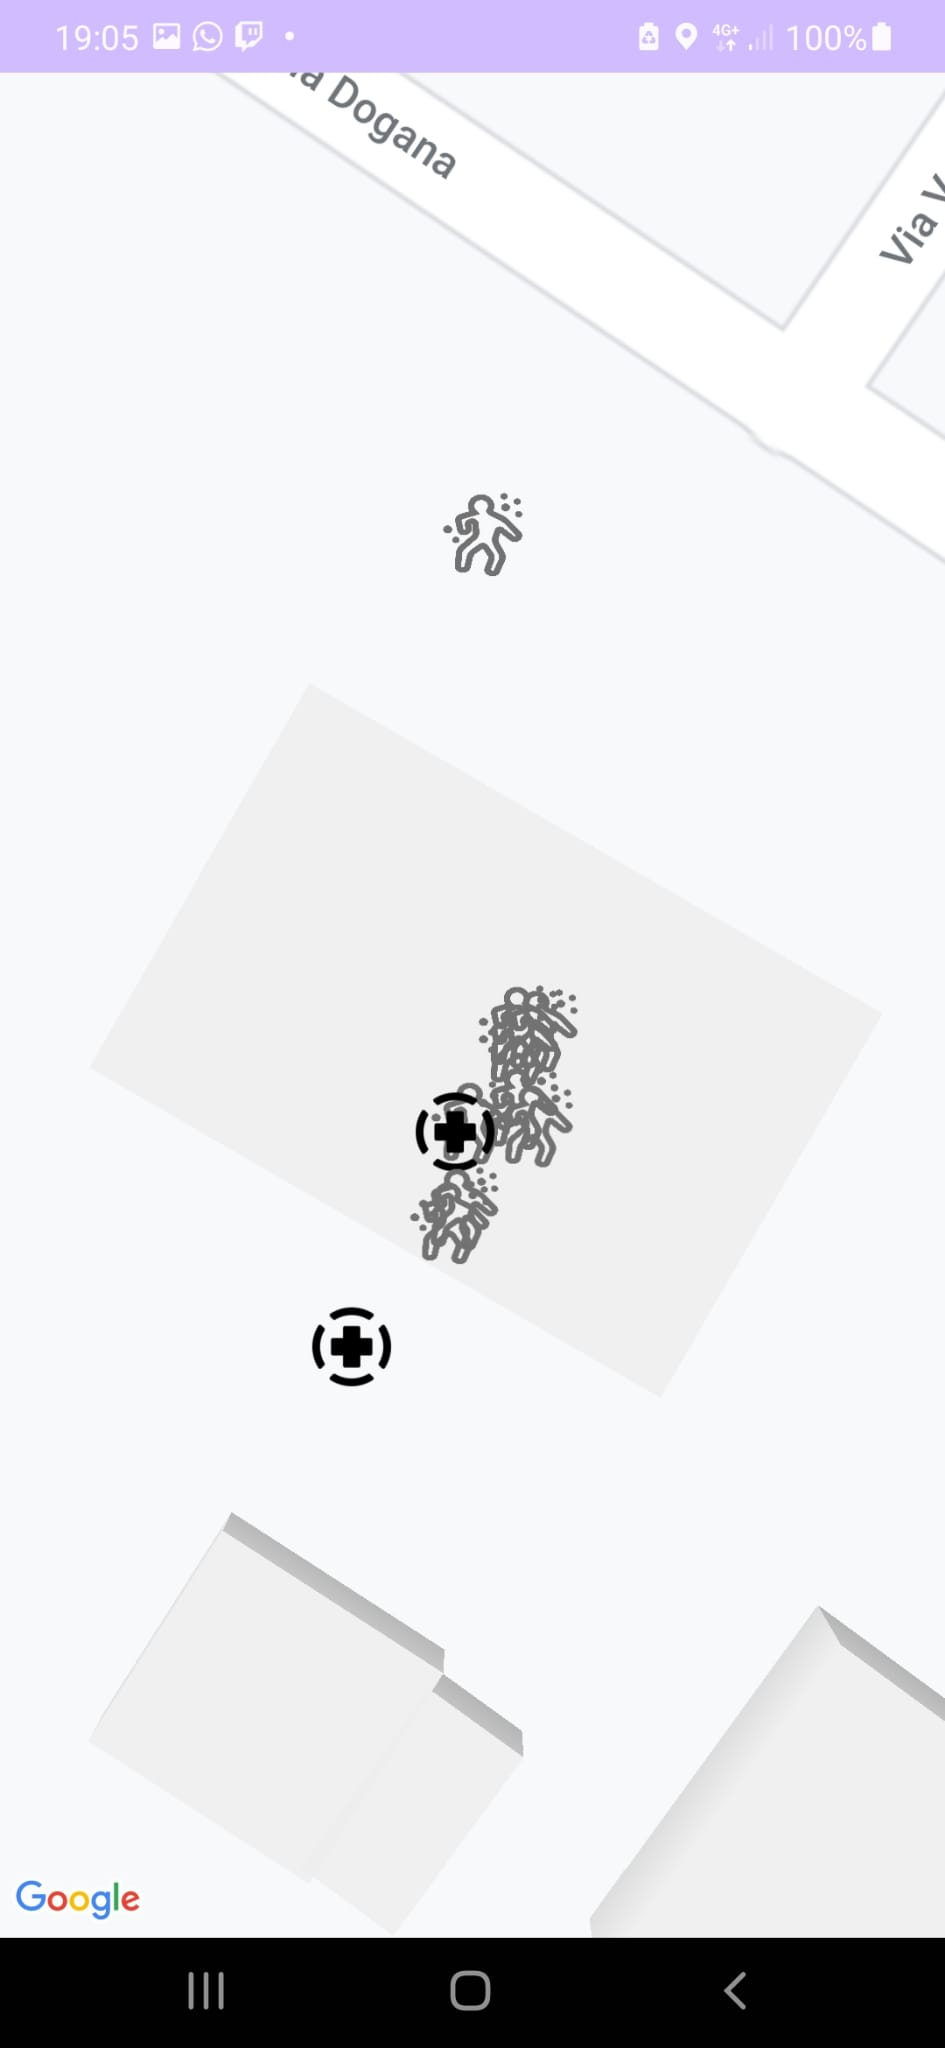
\includegraphics[width=2cm]{fig/map.jpg} 
    \caption{In the map interface, 
    the user can see the position of
    SAR and PV devices.}
\end{figure}
\begin{figure}[H]
    \center
    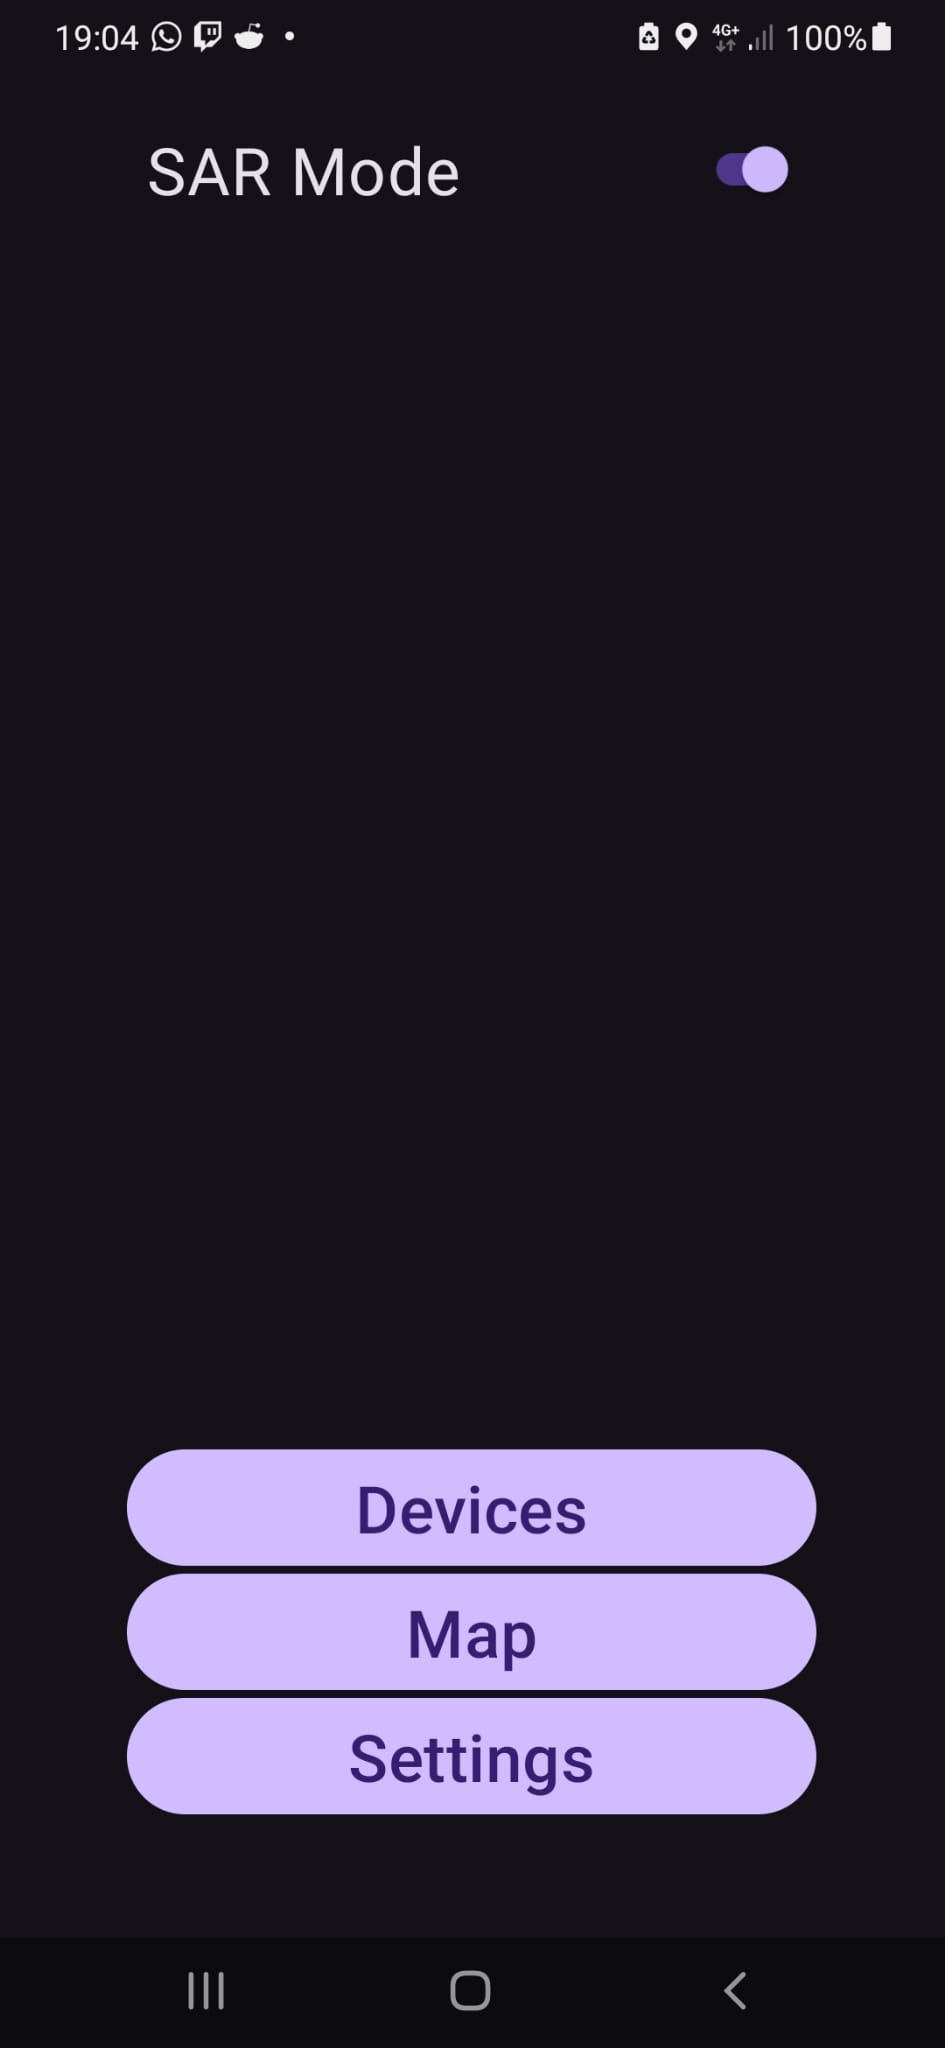
\includegraphics[width=2cm]{fig/main.jpg}
    \caption{In the main view a SAR user can
    open the map or a list of detected devices.
    Both a SAR and a PV user can open the settings
    to edit their personal information.}
\end{figure}
\end{multicols}
The application is designed to let only SAR 
operators open the map interface and the device
list. While both SAR and PV users can edit their
personal information.
In the map view, the user can select a device to
display its information.
\subsection{Data Sharing}
The application uses a gossip protocol to share
data along the ad-hoc BLE network. This is done 
over a GATT service. The packet is in encoded in
CBOR format and contains the device's information
along with those of onother random device.
\subsection{Localization}
The application stores a number of 
distance-position pairs both detected from the
device with BLE and received from other devices.
This enables even a sigle moving device to
localize a victim exploiting its own position that
changes over time and is obtained from GPS.
\section{Results}
The application was able to detect the location of
a device within a 10 meter radius in an open field.
For devices with the application installed, the
localization error was reduced to the error of the
GPS.
\section{Conclusion}
A mobile application was developed to enhance the
localization of victims in emergency situations.
The application uses BLE technology to create an
ad-hoc network and trilateration to estimate the
victim's position.
Further improvements could be made to the
accuracy of the localization by using a more
advanced data selection algorithm for the 
gossip protocol and a more accurate or dynamic
path loss model.
\end{multicols}
\bibliographystyle{IEEEtran}
\bibliography{references}
\end{document}